\section{Обсуждение выводов}
По результатам эксперимента настоящего исследования сформирована итоговая сравнительна таблица ранее отобранных моделей. Сравнение производится как для развитых, так и для развивающихся рынков. Оценка модели происходит на основе ее способностей прогнозировать как цены, так и доходности на 1 рабочий день биржи.

Однако, исходя из имеющегося количества данных, а именно $15 \cdot 2 \cdot  2 \cdot 15 = 900$ значений, для удобства визуального восприятия производим дробление вида: компания; модель; ошибка. Подобная структура имеется как для доходностей и цен, так и для рынков Китая и США. Для начала смотрим на полученные результаты относительно цен на развитом рынке. После этого переключаемся на доходности. Далее аналогичным образом проходимся по развивающемуся рынку.

Подобный план представления полученного результата сформирован для более удобного восприятия читателем, так как большое количество данных почти всегда равно трудностям в понимании выводов.

\begin{figure}[H]
	\centering
	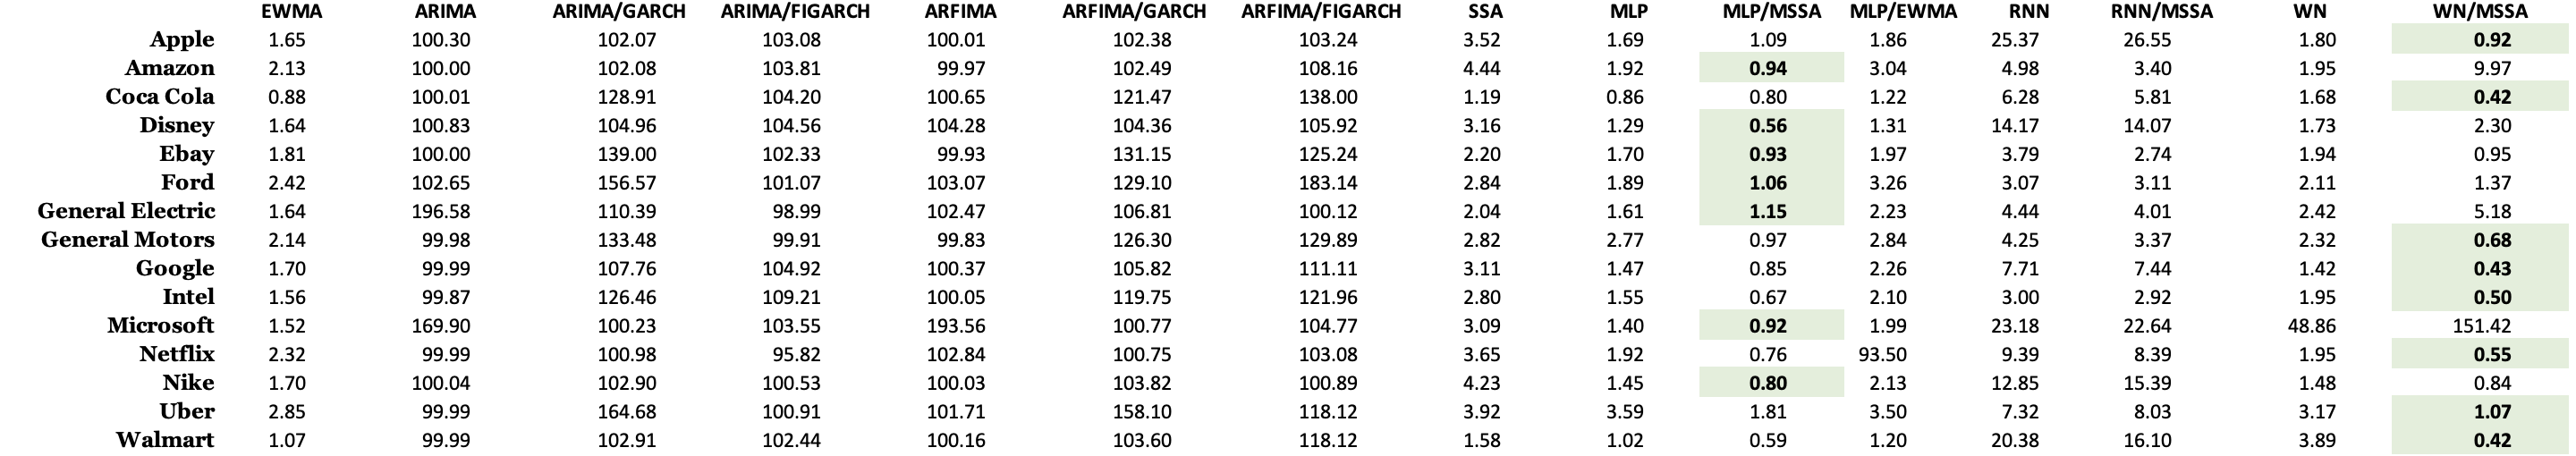
\includegraphics[width= 17cm]{./final tables/us_prices.png}
	\caption{Таблица итоговых значений WAPE (США, цены) в \%}
	\label{pic::final_table_us_prices}
\end{figure}

\noindent Исходя из полученных данных, видим, что в основном соревнование ведется между моделями Multilayer Perceptron (\myref{link::neural_networks}) в комбинации с отчисткой данных от шума посредством Multistage Singular Spectrum Analysis (\myref{link::mssa}) и Wavelet Network (\myref{link::wavelet_nets}). Интересно, что для большинства рассмотренных компаний WN + MSSA дает более точный прогноз на 1 рабочий день биржи, что наталкивает на гипотезу о превалировании или простом наличии доминантных частот в ценах на развитом рынке. Это и позволяет самообучающейся функции <<подгоняться>> (обучаться) именно на них, что дает частотно-временному анализу преимущество перед классическим подходом MLP. Данный вопрос достаточно интересен и требует более детального анализа, который производится в последующих работах автора настоящего исследования. Однако нельзя забывать и об успехах MLP + MSSA, ведь именно данная модель занимает второе место в прогнозе цен. В средних же величинах --- посредством усреднения для всех компаний --- у MLP + MSSA показатель WAPE равняется $1.08\%$, а у WM + MSSA $11.8\%$, что безусловно выводит MLP + MSSA на 1-ое место. Однако, вычислив средние по выделенным зеленым значениям, получаем WN + MSSA ($0.62\%$), а MLP + MSSA ($0.91\%$), что делает частотно-временную модель более точной в прогнозах. Отсюда нельзя сделать однозначный вывод о победе той или иной модели, так как они <<идут бок о бок>>, следовательно, необходимо в процессе построения прогнозного значения опираться на результат каждой из них. То есть для прогноза цен открытия рассмотренных компаний выявлены два победителя: MLP + MSSA и WN + MSSA.

Нельзя не заметить результаты статистических моделей --- ничего не думающих об имеющихся данных --- EWMA (\myref{link::ewma}) и SSA (\myref{link::ssa}). Данные модели не делают никаких предпосылок относительно анализируемых данных, однако ошибки их прогнозов не так далеки от лидеров данной гонки. Это наталкивает на мысль о возможном компромиссе относительно применяемой модели: если нужно максимальное качество (и при этом есть время), то WN + MSSA или MLP + MSSA, иначе (если необходим максимально быстрый ответ) EWMA или SSA. Рассмотренные только что 4 модели выделяют наиболее выдающиеся результаты, полученные, исходя из имеющихся данных. Другими словами, нельзя однозначно говорить о $100\%$-ой гарантии наличия доминантных частот в сигнале без дополнительного исследования. Но можно сформулировать гипотезу об этом. Также нельзя утверждать, что для остальных компаний этих же рынков результат будет аналогичным, так как все компании индивидуальны. Значит, \textit{основываясь на имеющихся данных рассмотренных компаний}, получаем максимальную точность у WN + MSSA и MLP + MSSA для развитого рынка. Далее идут EWMA и SSA.

Глядя на все эконометрические модели, видим, что их средняя ошибка для рассмотренных компаний составляем $112.07\%$, а фактические величины WAPE почти не опускается ниже $100\%$, что делает проанализированные модели практические непригодными для работы с финансовыми рядами рассмотренного типа (цены открытия). Однако лучшими моделями в данном блоке являются ARIMA и ARFIMA, дающие результат в среднем $100\%$ отклонение.

Относительно рекуррентных моделей типа RNN, RNN + MSSA нельзя сказать, что они совершенно непригодны для работы с временными рядами, однако, основываясь на \cite{transformers_are_useless_for_TSF}, видим, что все-таки временные ряды не то, где подобного рода модели имеют большое преимущество. Как уже говорилось ранее для успешной работы рекуррентной сети необходима задача обработка естественного языка, то есть --- набора слов/предложений, а не просто чисел, как в случае с анализом временных рядом, так как в тексте есть смысл, который и пытается <<вытащить>> модель.

Переходя к анализу доходностей для развитого рынка, сморим на полученную таблицу значений. Видим безоговорочную победу модели RNN + MSSA, что объясняется успешной очисткой данных от шума и последующим извлечением некоторого смысла из него посредством алгоритма RNN. Остальные модели --- все, кроме RNN --- показывают плохой результат, близкий к значениям эконометрических моделей на ценах развитого рынка. Из этого делаем вывод, что для рассмотренного набора доходностей имеющихся компаний почти одинаково плохо подходят как эконометрические, так и нейросетевые модели. Победителем в этой <<гонке>> является RNN + MSSA, однако нельзя забывать о примерах работы данной модели (\myref{link::rnn_module}), когде отчетливо показывается неспособность RNN семейства достаточно точно \footnote{Под словом <<точно>> имеется формирование среднего меньше, чем отклонение. Данное дополнение к имеющейся обученной модели позволяет достоверно оценивать финансовые риски.} предсказывать доходности. Таким образом, формально лидер определен, но подобный результат, им предоставляемый, не является валидным для практического применения и требует более тщательного анализа.
\begin{figure}[H]
	\centering
	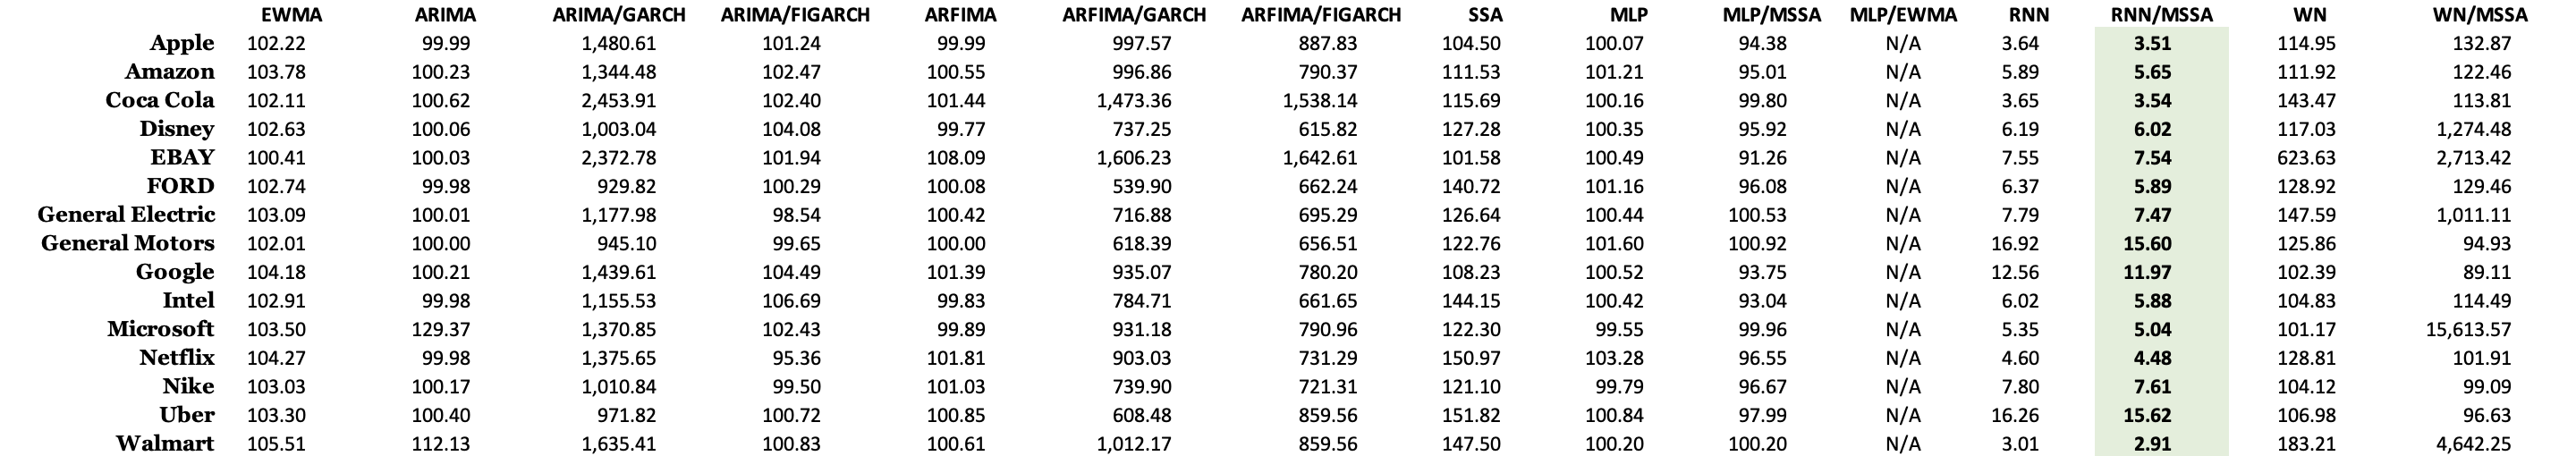
\includegraphics[width= 17cm]{./final tables/us_returns.png}
	\caption{Таблица итоговых значений WAPE (США, доходности) в \%}
	\label{pic::final_table_us_returns}
\end{figure}

\noindent Блок MLP + EWMA для доходностей не заполнялся, так как вычисление экспоненциального сглаживания доходностей для автора исследования не носит как практического, так и экономического смысла.

\begin{figure}[H]
	\centering
	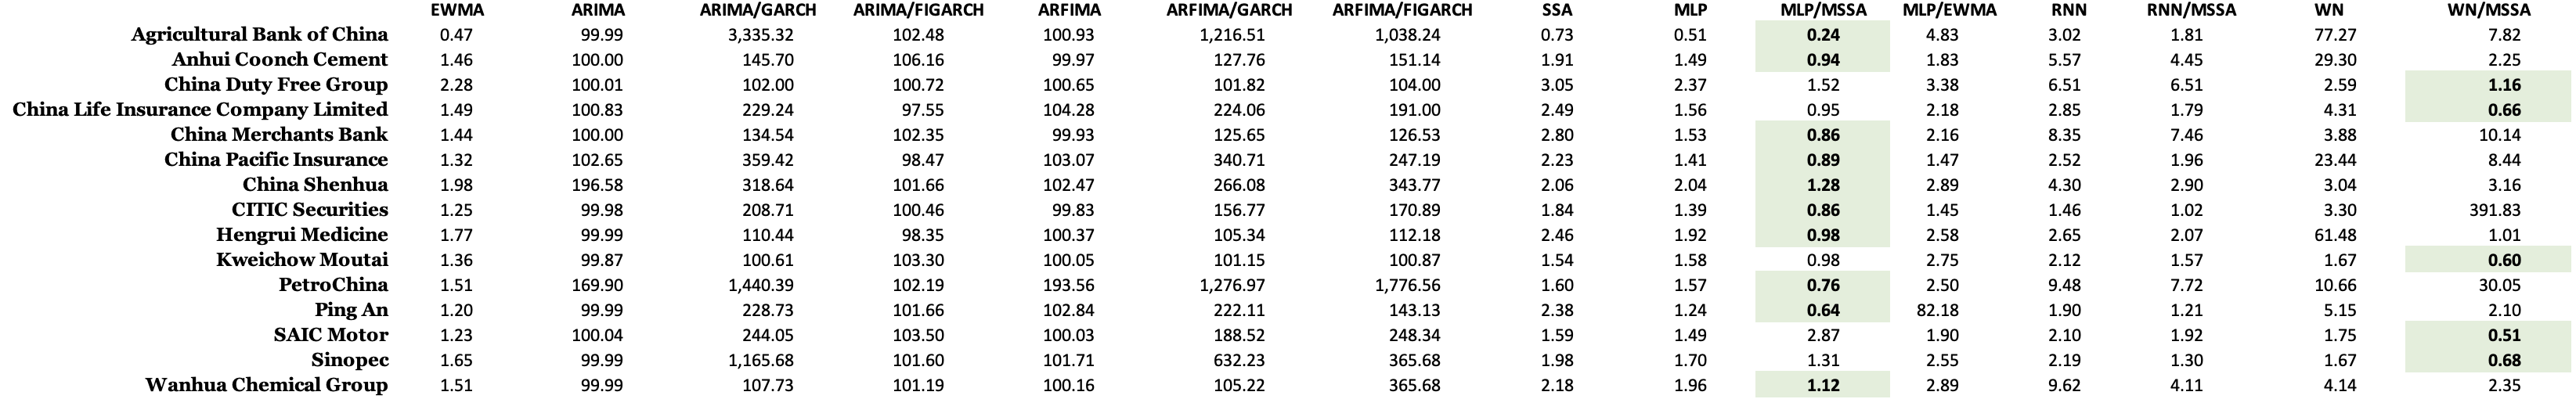
\includegraphics[width= 17cm]{./final tables/china_prices.png}
	\caption{Таблица итоговых значений WAPE (Китай, цены) в \%}
	\label{pic::final_table_china_prices}
\end{figure}


Переходим к блоку развивающегося рынка и аналогичным образом смотрим на показатели WAPE для цен. Ситуация очень похожа на только что рассмотренный развитый рынок: WN + MSSA и MLP + MSSA конкурируют друг с другом. Однако тут первенство все-таки остается за MLP + MSSA с достаточно большим перевесом. Среднее значение для MLP + MSSA равно $0.86\%$ (для выделенных зеленым цветом), а для WN + MSSA --- $0.72\%$, что аналогично показывает более точные прогнозы у WN + MSSA, однако уже на меньшем количестве компаний. Лидером соответственно становится MLP + MSSA (с оговоркой на наличие WN + MSSA, который старается дотянуться до своего оппонента).

Статистические модели аналогично показывают сравнимый с MLP + MSSA результат, не выдавая при этом каких-либо кардинальных различий между своей работой на развитом и развивающемся рынках. Это говорит об их стабильности (инвариантности) относительно самого поведения анализируемых величин.

Эконометрические модели в свою очередь в среднем дают $263.43\%$ отклонение, что делает их еще более непригодными моделирования временных рядов рассмотренных компаний. Однако лучшими на данный момент являются ARIMA + FIGARCH и ARFIMA, дающие в среднем $104.38\%$-ое отклонение. В любом случае, данные модели не применимы к реальной жизни из-за слишком большой ошибки.

Ситуация с применением алгоритма MSSA остается аналогичной, так как очистка рассмотренных данных дает прирост к качеству прогноза той или иной модели. Соответственно алгоритм MSSA в среднем (тут важно помнить о комбинации WN и MSSA) дает более хороший результат, что привлекает более пристальное внимание к принципу его работы \cite{kuang2020efficient}. 

\noindent Далее смотрим на полученные результаты для доходностей на развивающемся рынке:

\begin{figure}[H]
	\centering
	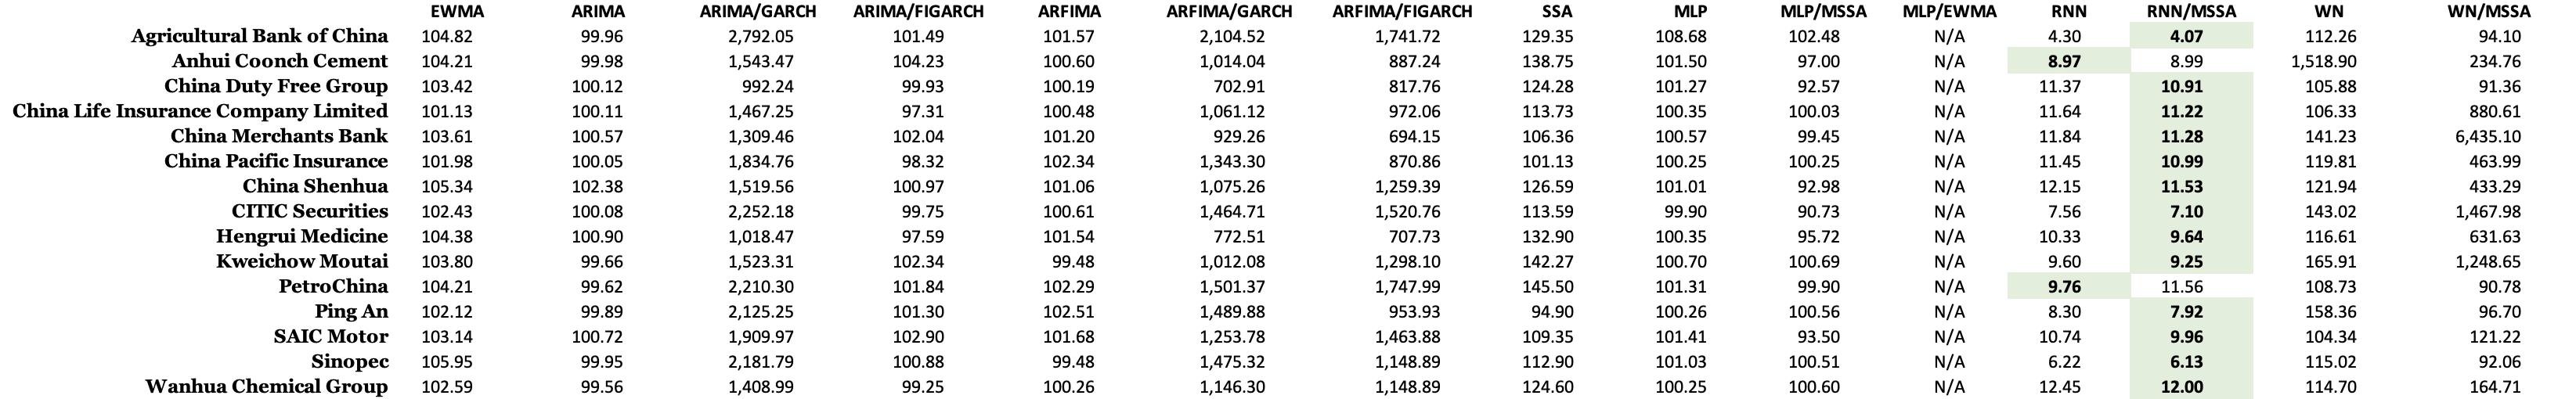
\includegraphics[width= 17cm]{./final tables/china_returns.png}
	\caption{Таблица итоговых значений WAPE (Китай, доходности) в \%}
	\label{pic::final_table_china_returns}
\end{figure}

\noindent Как и ожидалось результат повторяется, то есть RNN + MSSA показывают лучшие значения для всех имеющихся моделей. Исключением при этом являются компаниии Anhui Coonch Cement и Kweichow Moutai, для которых RNN дает результат лучше, чем RNN + MSSA. Это пример того, что алгоритм MSSA не является универсальным средством и может давать не только улучшение, но и ухудшение посредством случайного удаления информации о важных показателях сигнала, содержащих тренд. Все остальные модели аналогичным образом показывают результат около или даже выше $100\%$-ого отклонения, что автоматические делает их неприменимыми к реальности.

Подводя итог блоку анализа результатов, выделяем несколько наиболее важных вещей, сформулированных в ходе эксперимента: 1) WAPE для прогнозов цен заметно меньше почти для всех (за исключением эконометрических) моделей, чем WAPE для доходностей. То есть для имеющихся данных проще предсказывать именно цены 2) MSSA + MLP, а также MSSA + WN являются лидерами в области прогнозирования цен для проанализированных компаний 3) MSSA + RNN является лучшей для предсказания доходностей, однако ее результаты не являются допустимыми для применения к реальности в силу достаточно большой ошибки относительно сравнительно малого среднего значения прогноза 4) Эконометрические модели плохи как для прогнозов цен, так и для прогнозов доходностей (опять же вывод происходит из имеющихся данных и не носит $100\%$-ый характер) 5) Алгоритма очистки от шума MSSA показывает отличный результат, добавляя почти ко всем моделям в точности прогноза как цен, так и доходностей. Исключением тут модель WN + MSSA. Факт успешного применения MSSA объясняется наличием большого количества шума в имеющихся данных. То есть моделям лучше <<настраиваться>> на чистые значения того или иного показателя, в нашей терминологии --- тренд.

Дополнением к данному блоку служит формулировка гипотезы, проверяемой автором в будущих исследованиях:
\begin{uncertainty}
	Для цен активов развитого финансового рынка характерно наличие большего количества частотных составляющих, чем для развивающегося.
\end{uncertainty}
